\chapter{Implementacija i korisničko sučelje}
		
		
		\section{Korištene tehnologije i alati}
		
			Za međusobnu komunikaciju unutar tima koristili smo aplikacije WhatsApp i Discord. \textbf{\textit{WhatsApp}} je popularna platforma koja omogućava korisnicima slanje poruka i medijskih datoteka te obavljanje glasovnih/video poziva. \textbf{\textit{Discord}} je aplikacija za stvaranje servera na kojima članovi mogu komunicirati putem poruka i poziva. 
			
			Za modeliranje UML dijagrama koristili smo \textbf{\textit{Astah UML}}, alat koji omogućava korisnicima da kreiraju različite vrste UML dijagrama. Za pripremu i uređivanje dokumentacije koristili smo \textbf{\textit{TeXstudio}}, specifično prilagođeno okruženje za učinkovit rad s LaTeX sustavom.
			
			Po pitanju baze podataka i svega vezanog uz nju koristili smo nekoliko alata. Alatom \textbf{\textit{ERDplus}}, popularnim online alatom za izradu ER dijagrama, modelirali smo ER dijagram. Sama baza podataka temeljena je na \textbf{\textit{PostgreSQL}}-u, poznatom sustavu za upravljanje bazama podataka. \textbf{\textit{Firebase}} je platforma koja nam služi za pohranu slika koje organizatori postavljaju uz svoje događaje. Alat \textbf{\textit{Liquibase}} koristili smo za upravljanje promjenama u shemi baze podataka.
			
			Za ispitivanje komponenti iskoristili smo \textbf{\textit{JUnit}}, okvir za testiranje osmišljen za podršku automatskom testiranju Java aplikacija, i \textbf{\textit{Mockito}}, koji nam je poslužio za stvaranje lažnih, mock objekata. Za ispitivanje sustava upotrijebili smo \textbf{\textit{Selenium IDE}}, alat koji omogućuje snimanje, uređivanje i reprodukciju testova jednostavnim klikanjem i snimanjem korisničkih radnji na web stranici.
			
			Za upravljanje izvornim kodom primijenili smo sustav \textbf{\textit{Git}}, dok se sam kod nalazi na \textbf{\textit{GitHub}} platformi unutar udaljenog repozitorija. GitHub je jedna od najpoznatijih web platformi koja pruži usluge za upravljanje projektima temeljenima na Git sustavu.  
			
			Naposljetku, za izradu aplikacije upotrijebili smo mnogo različitih alata. Za frontend smo koristili \textbf{\textit{React.js}} uz \textbf{\textit{JavaScript}}, \textbf{\textit{Vite}} te \textbf{\textit{Material UI}}. React.js je popularna JavaScript biblioteka koja se koristi za izgradnju korisničkih sučelja u web aplikacijama. Vite je alat čija je osnovna svrha pojednostaviti i ubrzati razvoj web aplikacija. Material UI je poslužio za dizajniranje osnovnih komponenti frontenda. Za backend smo koristili \textbf{\textit{Javu}} i \textbf{\textit{Spring Boot}}, okvir za izgradnju Java aplikacija temeljenih na Springu, a koji je posebno koristan jer omogućuje programerima da se fokusiraju na poslovnu logiku aplikacije umjesto na konfiguraciju i upravljanje okolinom
			
			Deployment frontenda, backenda te baze podataka postigli smo uz pomoć platforme \textbf{\textit{Render}} koja služi za deployment i hosting web aplikacija. 
			
			\par\noindent\rule{\textwidth}{0.4pt}
			
				\begin{itemize}
					\item \footnotesize Whatsapp		\url{https://www.whatsapp.com/}
					\item \footnotesize Discord			\url{https://discord.com/}
					\item \footnotesize Astah UML		\url{https://astah.net/products/astah-uml/}
					\item \footnotesize TeXstudio		\url{https://www.texstudio.org/}
					\item \footnotesize ERDplus		\url{https://erdplus.com/}
					\item \footnotesize PostgreSQL		\url{https://www.postgresql.org/}
					\item \footnotesize Firebase		\url{https://firebase.google.com/}
					\item \footnotesize Liquibase		\url{https://www.liquibase.org/}
					\item \footnotesize JUnit			\url{https://junit.org/junit5/}
					\item \footnotesize Mockito		\url{https://site.mockito.org/}
					\item \footnotesize Selenium IDE		\url{https://www.selenium.dev/selenium-ide/}
					\item \footnotesize Git				\url{https://git-scm.com/}
					\item \footnotesize GitHub		\url{https://github.com/}
					\item \footnotesize React.js			\url{https://reactjs.org/}
					\item \footnotesize Vite			\url{https://vitejs.dev/}
					\item \footnotesize JavaScript		\url{https://www.javascript.com/}
					\item \footnotesize Material UI			\url{https://mui.com/}
					\item \footnotesize Java				\url{https://www.java.com/en/}
					\item \footnotesize SpringBoot			\url{https://spring.io/projects/spring-boot/}
					\item \footnotesize Render			 \url{https://render.com/}

				\end{itemize}

			
			
			
			\eject 
		
	
		\section{Ispitivanje programskog rješenja}
			
			U ovom poglavlju usredotočili smo se na testiranje programskog rješenja testirajući cijeli sustav, ali i komponente istog. Tijekom ispitivanja komponenti sustava korišteni su JUnit za izvršavanje testova te Mockito za stvaranje mock objekata korištenih u testiranju. Selenium IDE korišten je u ispitivanju sustava te nam je omogućio brzo i precizno provjeravanje funkcionalnosti web aplikacije.
			
			\subsection{Ispitivanje komponenti}
			
			U poglavlju o ispitivanju komponenti, razvijeni su i izvršeni testovi kako bi se osigurala kvaliteta i funkcionalnost komponenata sustava, a istovremeno se time osigurava pouzdanost i održivost koda. U nastavku su prikazani primjeri nekoliko testova koji su implementirani kao dio ispitivanja komponenti sustava:

			\textbf{Test sortiranja i ispisivanja događaja} provjerava ispravnu funkcionalnost sortiranja događaja prema određenom filtru, u ovom slučaju prema vremenu početka događaja. Također testirano je izlistavanje događaja, je li broj događaja jednak očekivanom broju. Korišten je JUnit za pisanje i izvršavanje testova te Mockito za stvaranje mock objekta i postavljanje očekivanja.


			\textbf{Test registracije korisinika} ispituje uspješnost registracije korisnika. Također se koriste Mock objekti koji simuliraju ponašanje komponenti tijekom registracije. Prikazana su dva testa, u jednom se testira registracija koja je uspješa, u drugom se testira neuspješna registracija korisnika.

			U nastavku su još prikazani sljedeći testovi: \textbf{Test slanja e-maila}, \textbf{Test spremanja recenzije}, \textbf{Test spremanja zainteresiranosti}. Oni redom provjeravaju točnost slanja e-maila, ispravnu funkcionalnost spremanja recenzije i zainteresiranosti. U navedenim testovima se također koriste spomenute tehnologije za provjeravanje ispravnosti. Osim testova, prikazano je i njihovo izvođenje te rezultat izvođenja.
			
			\begin{figure}[H]
				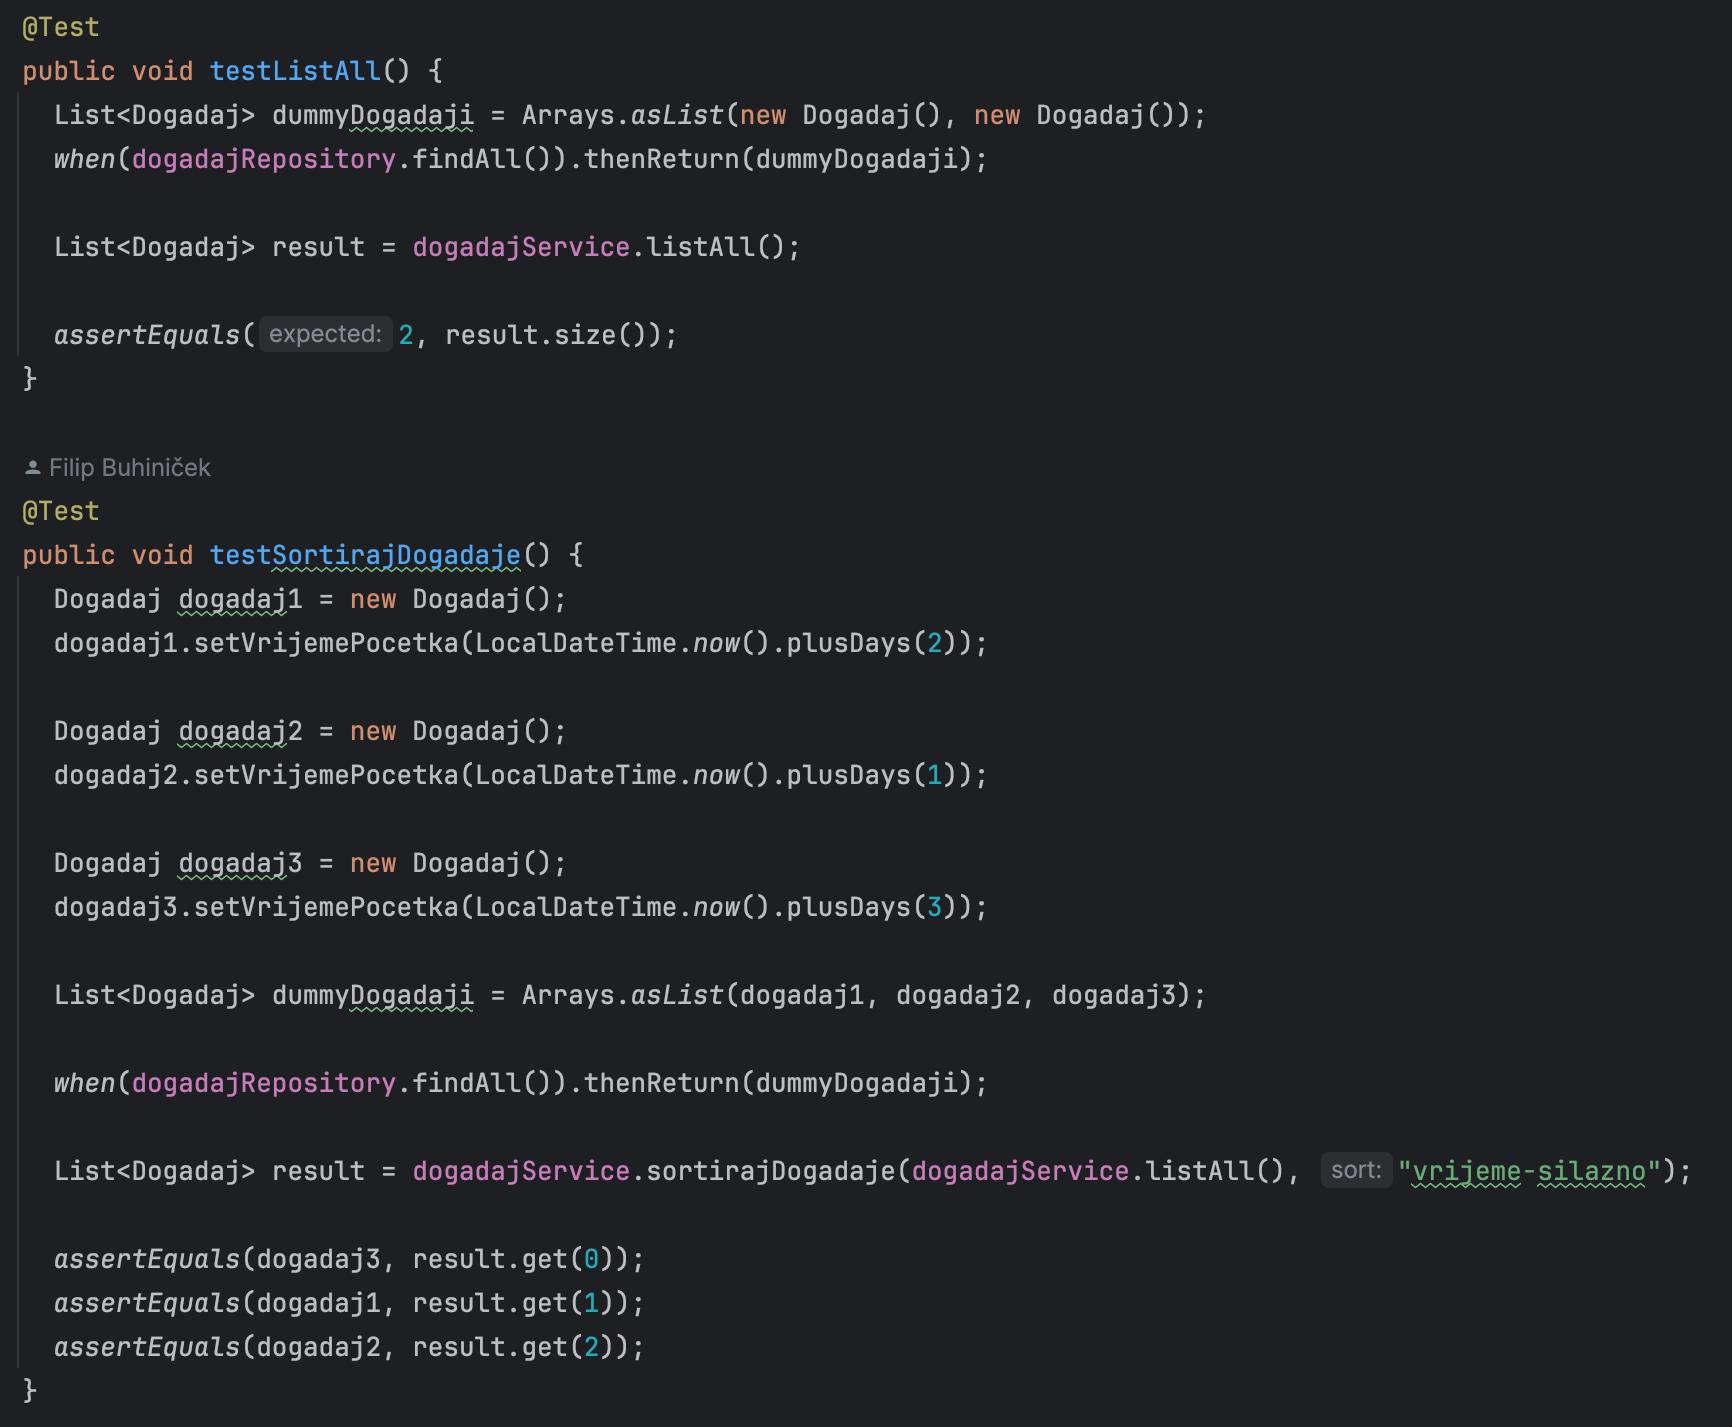
\includegraphics[scale=0.45]{testovi/dogadajTest.png}
				\centering
				\caption{Test za sortiranje i ispisivanje događaja}
				\label{fig:promjene}
			\end{figure}
			
			
			\begin{figure}[H]
				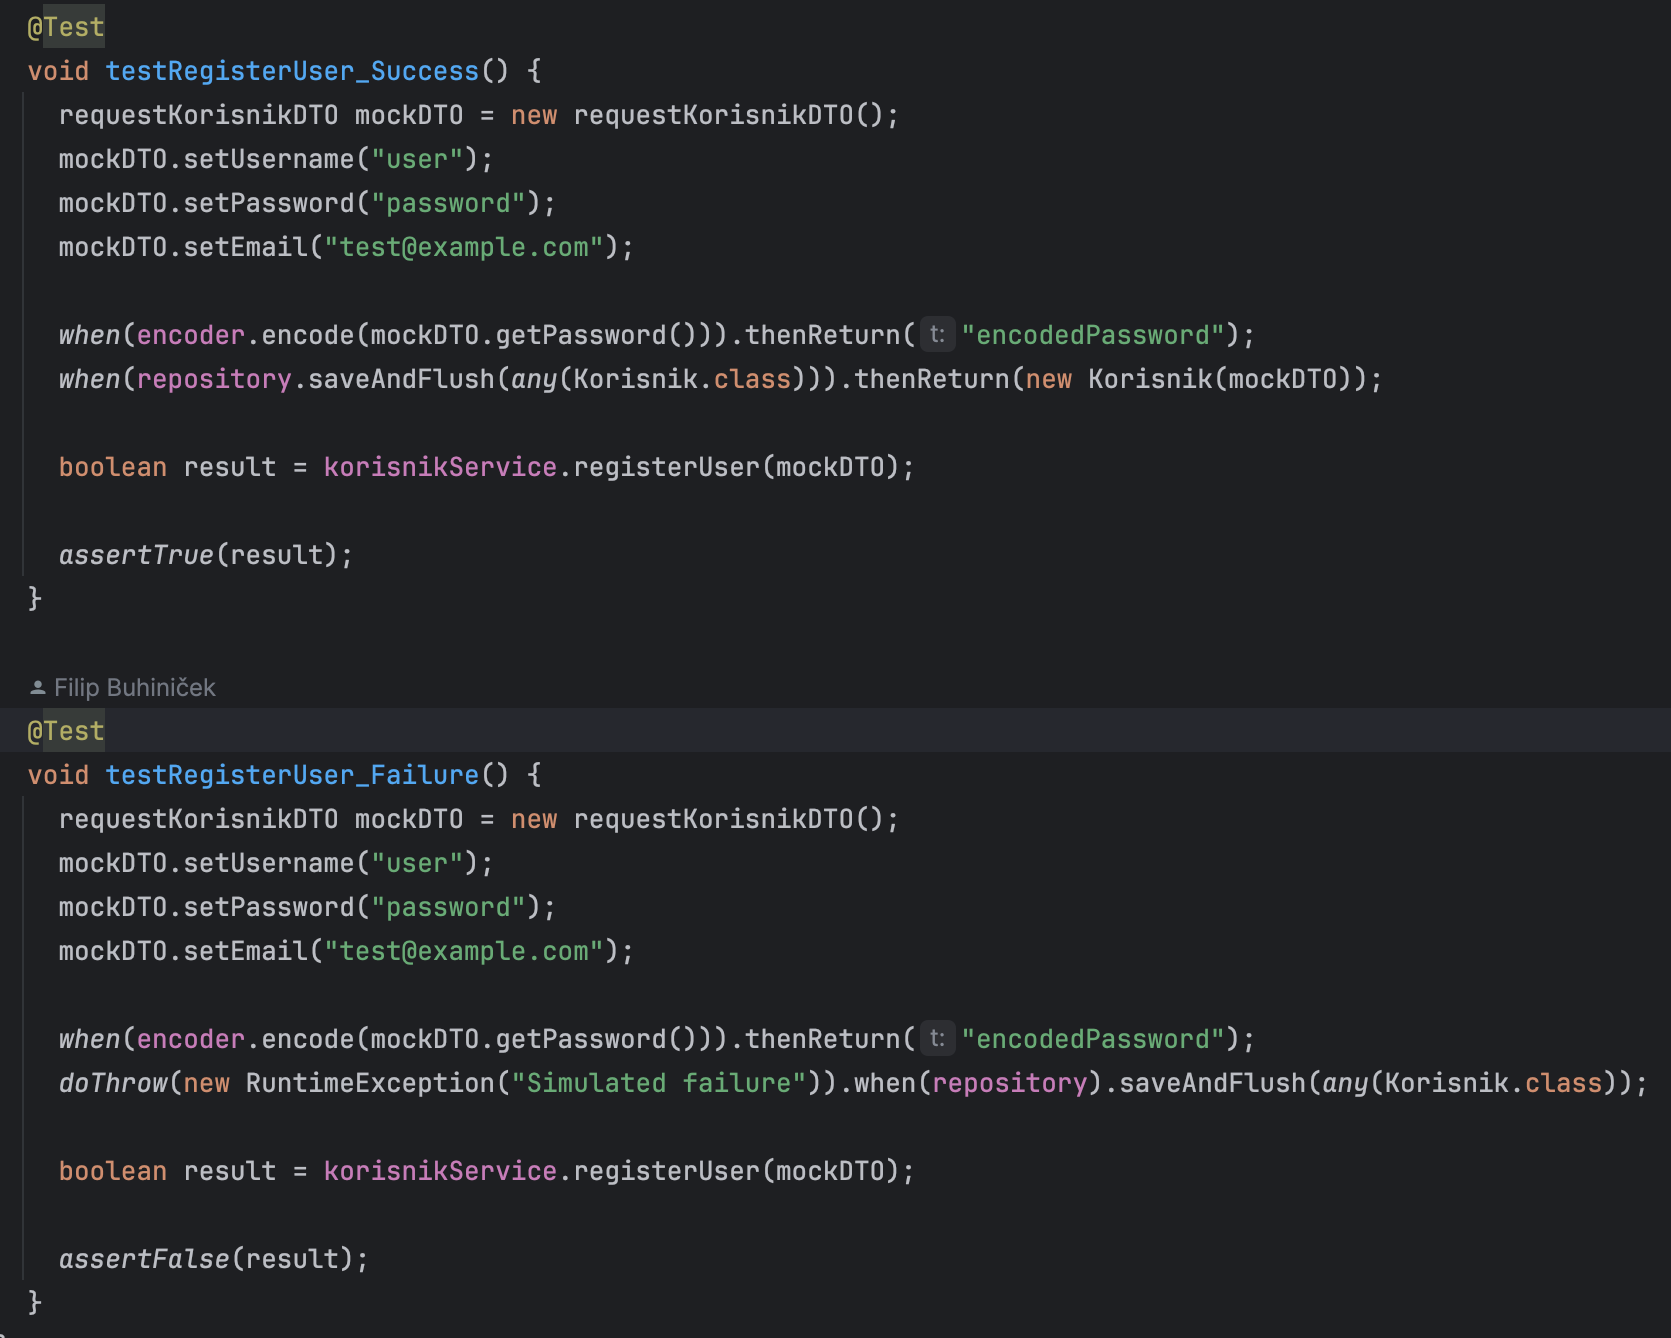
\includegraphics[scale=0.45]{testovi/korisnikTest.png}
				\centering
				\caption{Test registracije korisnika}
				\label{fig:promjene}
			\end{figure}
			
			
			
			\begin{figure}[H]
				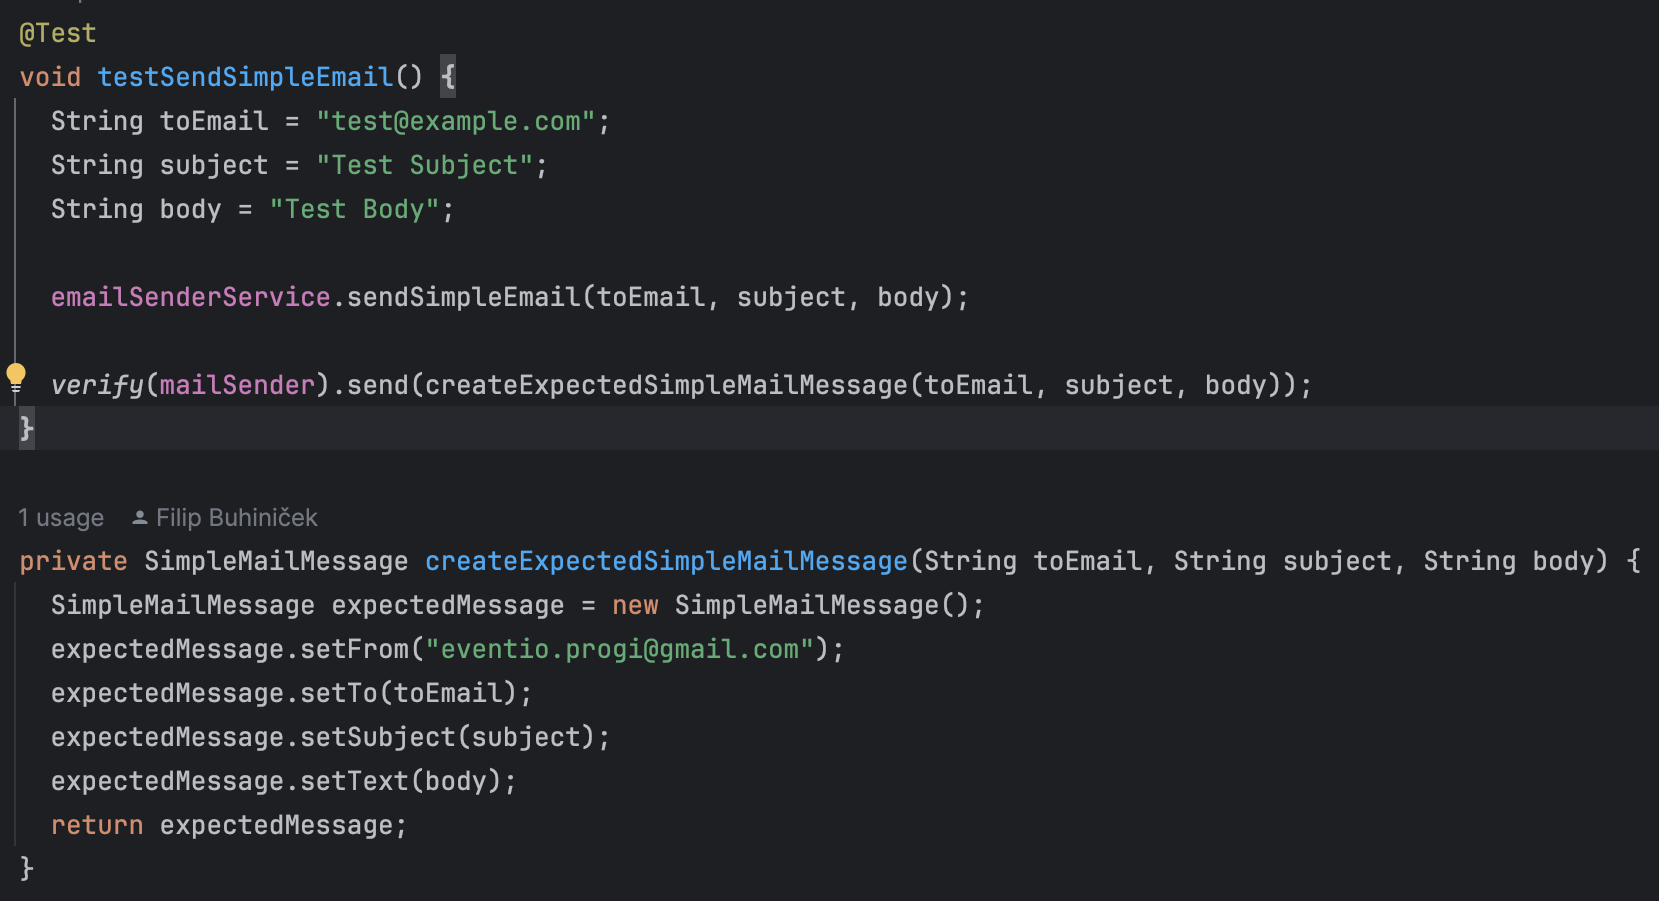
\includegraphics[scale=0.45]{testovi/emailTest.png}
				\centering
				\caption{Test slanja e-maila}
				\label{fig:promjene}
			\end{figure}
			
			\begin{figure}[H]
				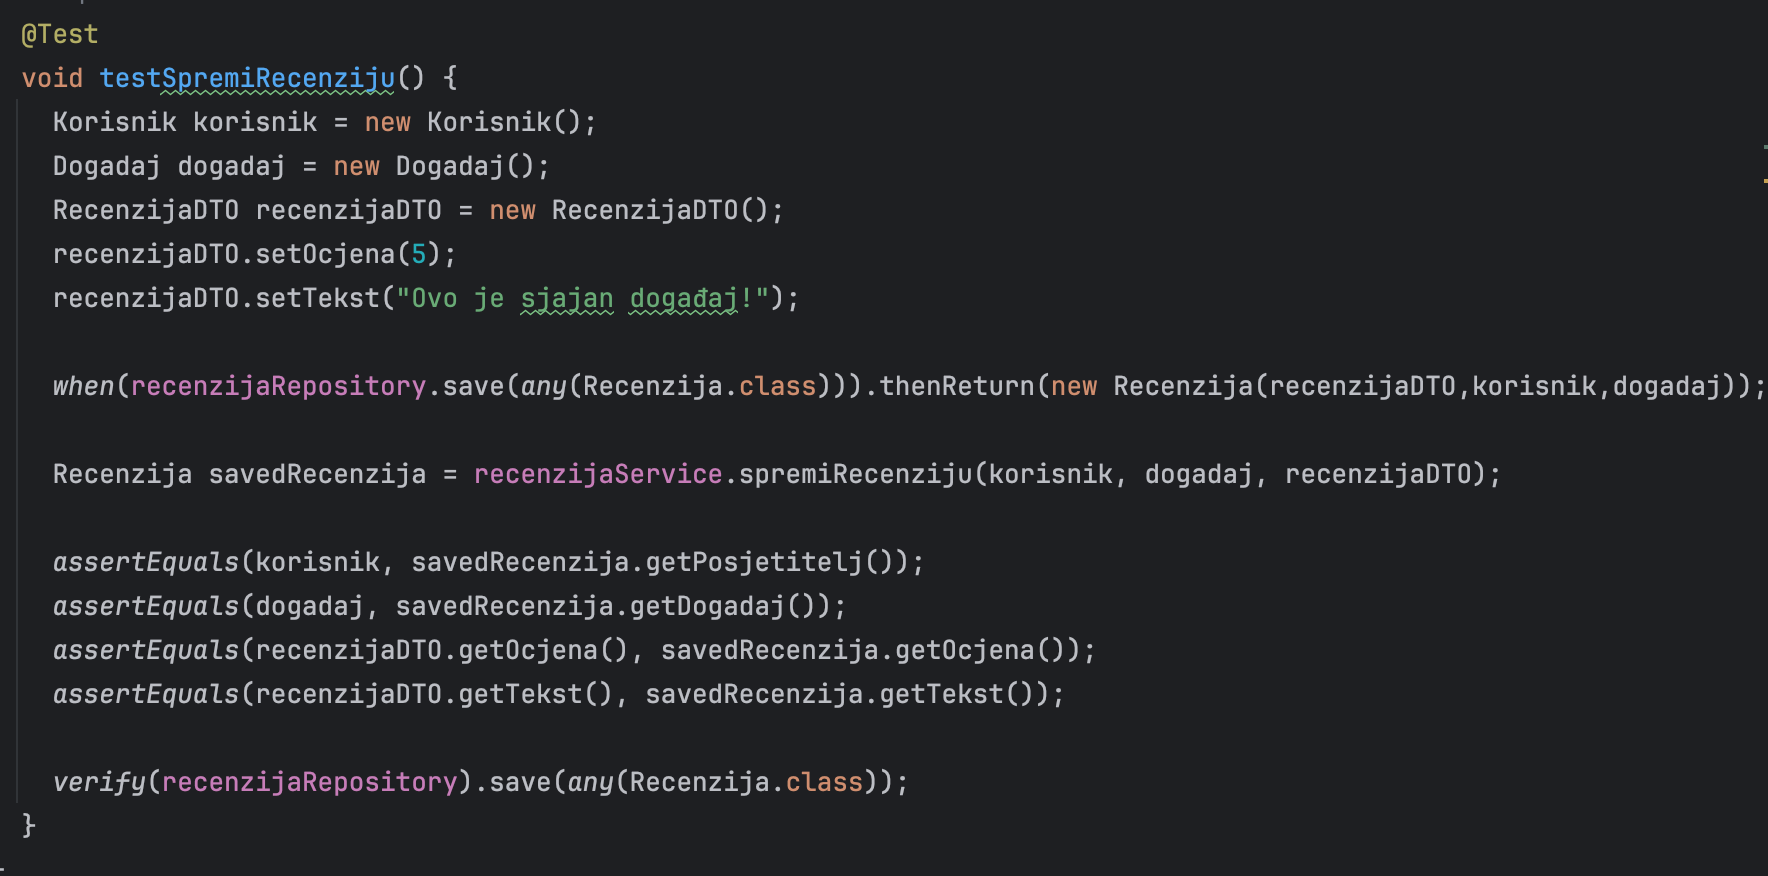
\includegraphics[scale=0.45]{testovi/recenzijeTest.png}
				\centering
				\caption{Test spremanja recenzije}
				\label{fig:promjene}
			\end{figure}
			
			\begin{figure}[H]
				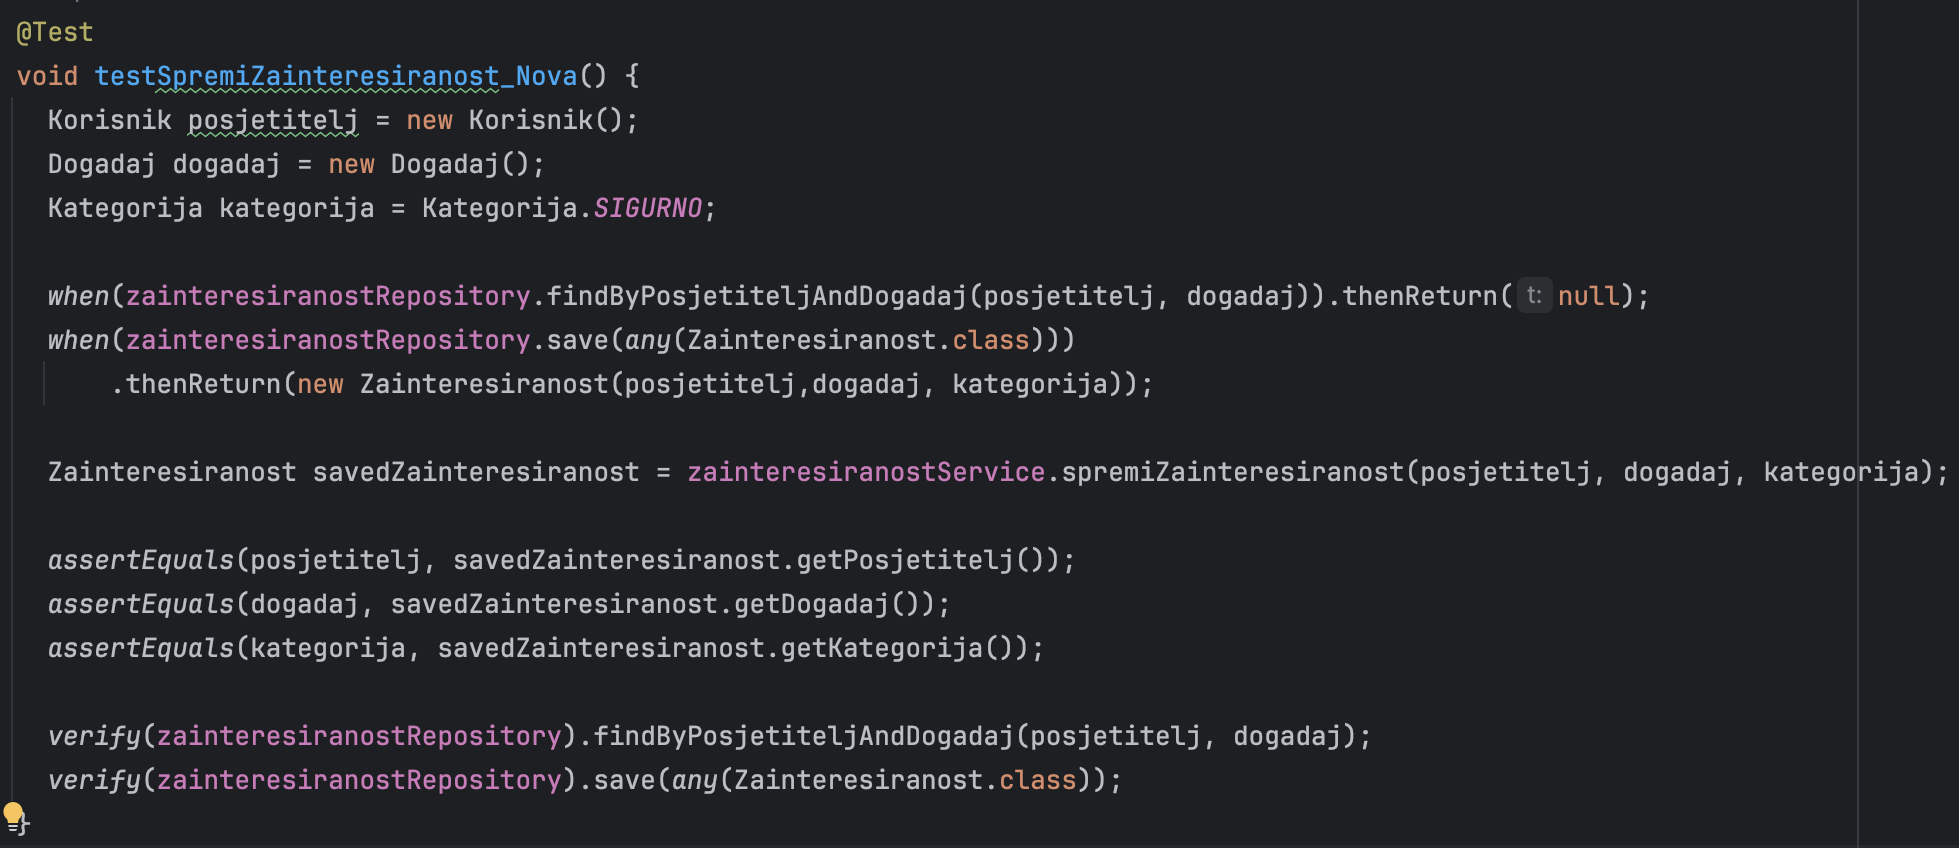
\includegraphics[scale=0.45]{testovi/zainteresiranostTest1.png}
				\centering
				\caption{Test spremanja nove zainteresiranosti}
				\label{fig:promjene}
			\end{figure}
			
			\begin{figure}[H]
				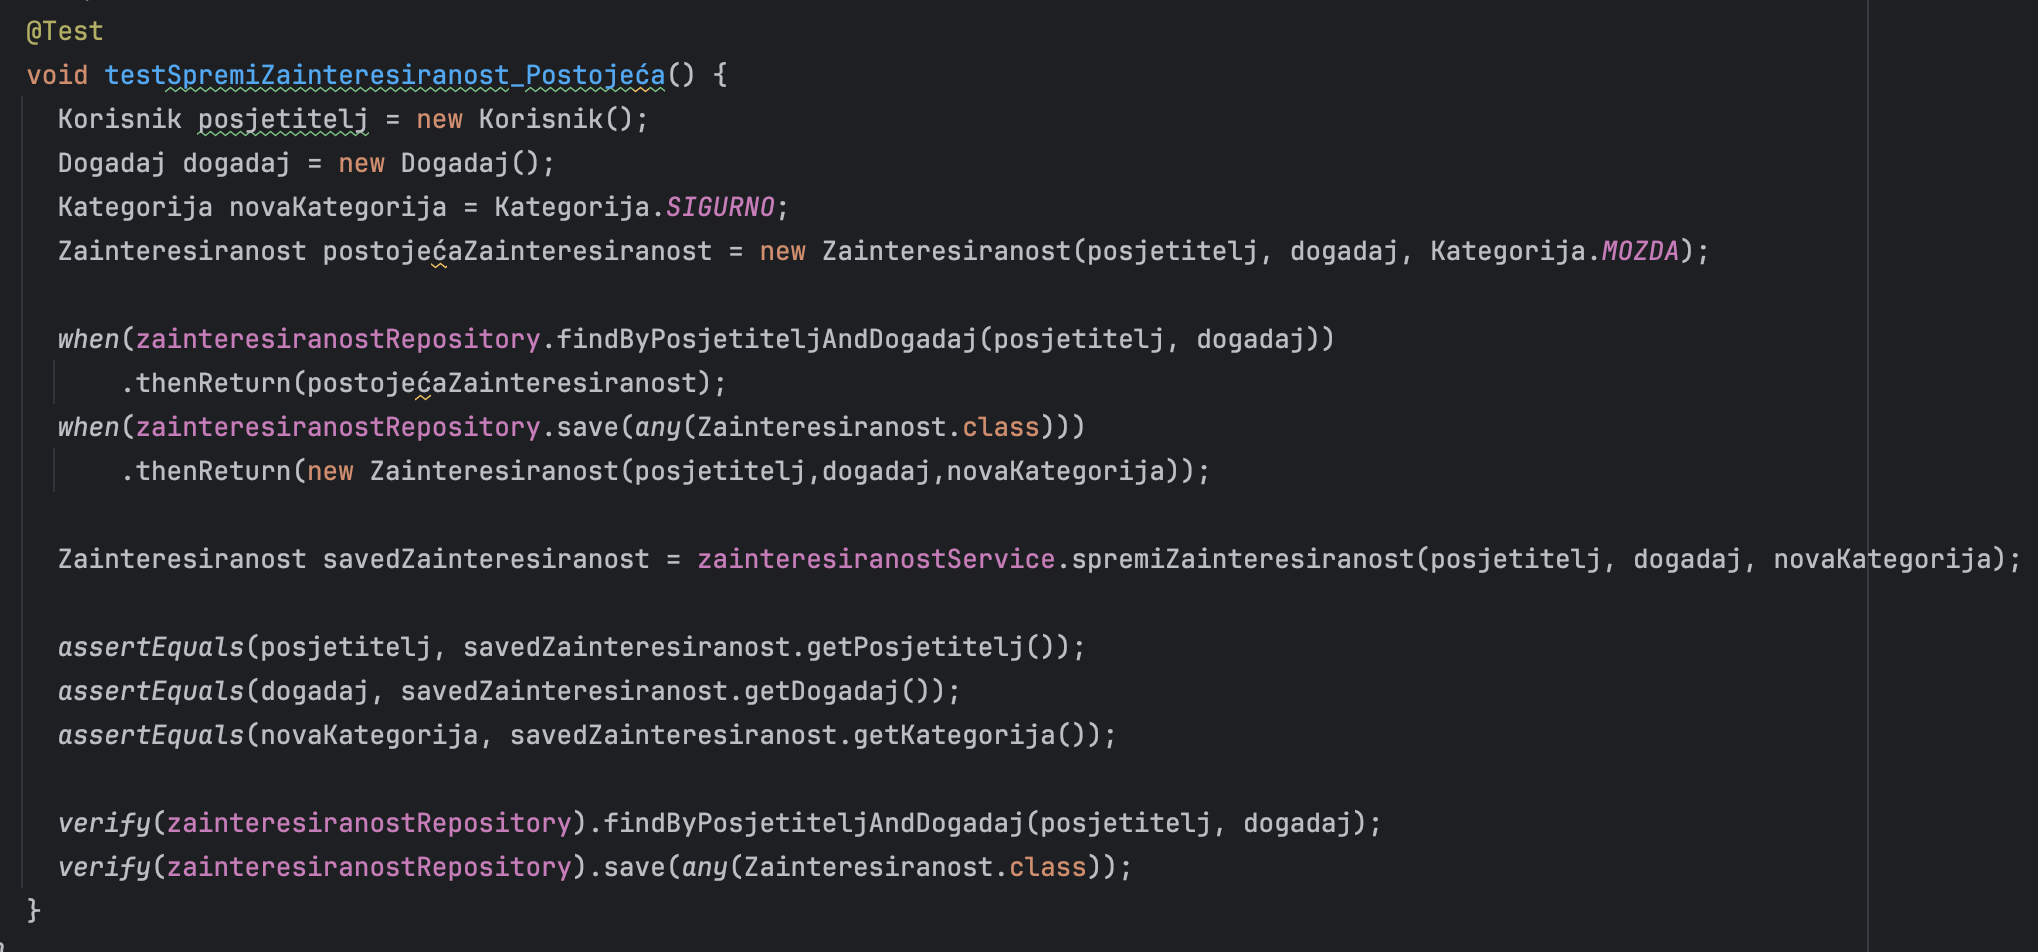
\includegraphics[scale=0.45]{testovi/zainteresiranostTest2.png}
				\centering
				\caption{Test spremanja postojeće zainteresiranosti}
				\label{fig:promjene}
			\end{figure}
			
				\begin{figure}[H]
				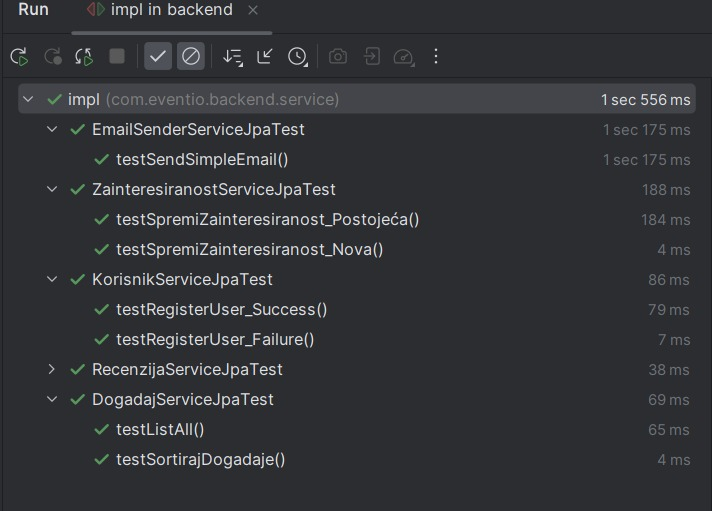
\includegraphics[scale=0.45]{testovi/unit_testovi.jpeg}
				\centering
				\caption{Izvršavanje i rezultati testova}
				\label{fig:promjene}
			\end{figure}
			
			
			\subsection{Ispitivanje sustava}
			
			U procesu ispitivanja sustava koristili smo Selenium IDE koji nam je omogućio precizno i brzo testiranje funkcionalnosti web aplikacije. Selenium IDE predstavlja moćan alat za testiranje web aplikacija te se istovremeno olakšava proces automatizacije. \newline Na sljedećim slikama prikazani su ispitni slučajevima kojima smo testirali funkcionalnost aplikacije. \textbf{Test prijave organizatora} provjerava uspješnost prijave korisnika koji je organizator. \textbf{Test stvaranja novog događaja} provjerava funkcionalnost stvaranja novog događaja sa svim postavkama. Prikazano je i izvršavanje \textbf{Testa promjene cijene pretplate} i \textbf{Testa stvaranja nove recenzije}.
			
			\begin{figure}[H]
				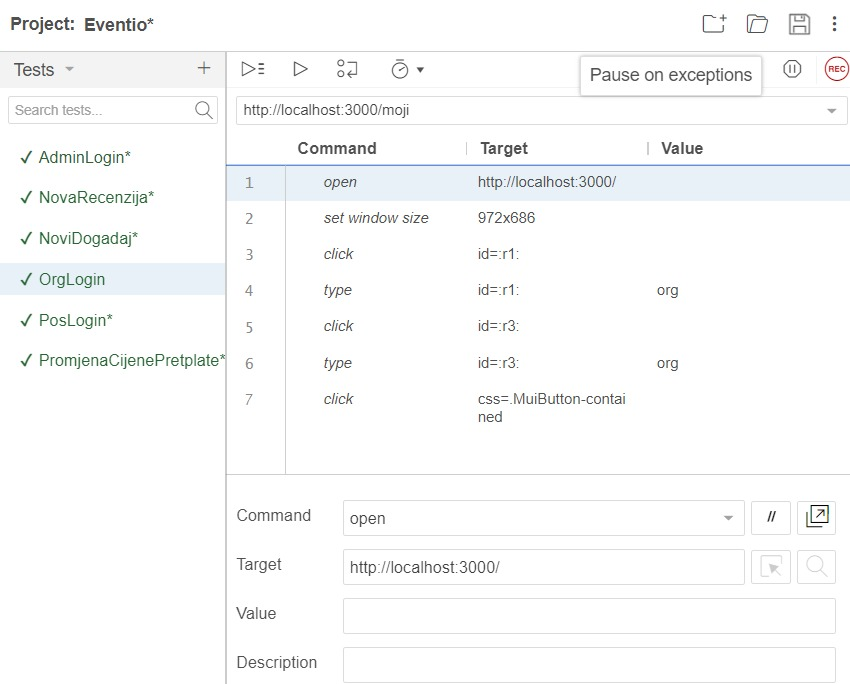
\includegraphics[scale=0.45]{testovi/selOrgLogin.jpeg}
				\centering
				\caption{Test prijave organizatora}
				\label{fig:promjene}
			\end{figure}
			
			\begin{figure}[H]
				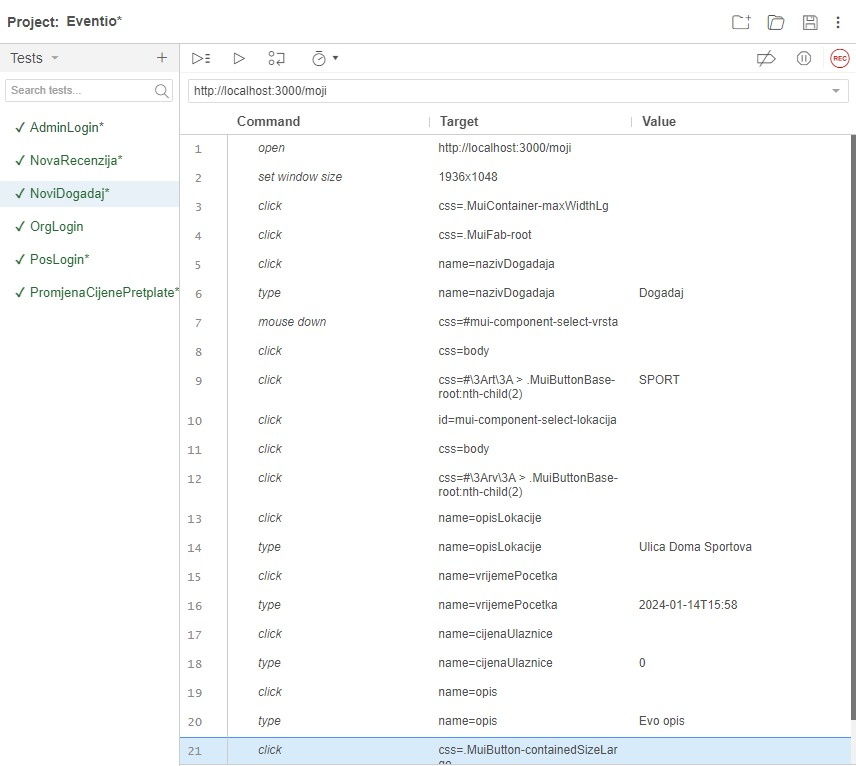
\includegraphics[scale=0.45]{testovi/selNoviDogadaj.jpeg}
				\centering
				\caption{Test stvaranja novog događaja}
				\label{fig:promjene}
			\end{figure}
			
			\begin{figure}[H]
				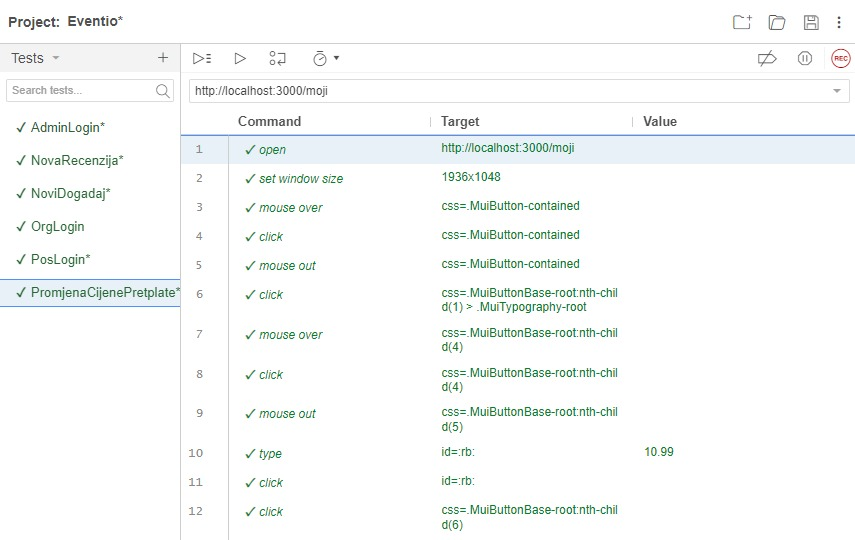
\includegraphics[scale=0.45]{testovi/selPretplata.jpeg}
				\centering
				\caption{Test promjena cijene pretplate}
				\label{fig:promjene}
			\end{figure}
			
			\begin{figure}[H]
				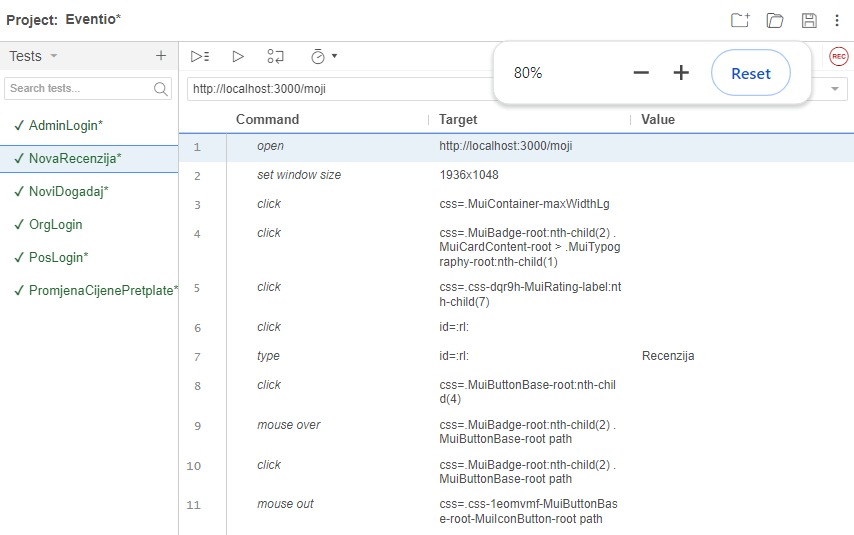
\includegraphics[scale=0.45]{testovi/selRecenzija.jpeg}
				\centering
				\caption{Test stvaranje nove recenzije}
				\label{fig:promjene}
			\end{figure}
			
		
		
		\section{Dijagram razmještaja}
			
			Dijagrami razmještaja opisuju topologiju sklopovlja i programsku potporu koja se koristi u implementaciji sustava u njegovom radnom okruženju. Korisnici pristupaju web aplikaciji putem web preglednika na svojim osobnim računalima. Arhitektura sustava temelji se na jasno odvojenim slojevima: frontendu, backendu i bazi podataka. 
			Frontend poslužitelj posvećen je izvršavanju i posluživanju resursa vezanih uz korisničko sučelje. Backend poslužitelj fokusiran  je na izvršavanje poslovne logike, pružanje API-ja te komunikaciju s bazom podataka. Na ovom sloju obavljaju se operacije i logika sustava, pružajući funkcionalnosti koje podržavaju rad aplikacije. Baza podataka poslužitelj je posvećen upravljanju bazom podataka. Ovdje se nalazi sama baza podataka i sustav za pohranu i dohvat podataka.  Komunikacija između korisnika i poslužitelja odvija se preko HTTP veze.
			 
			 \begin{figure}[H]
			 	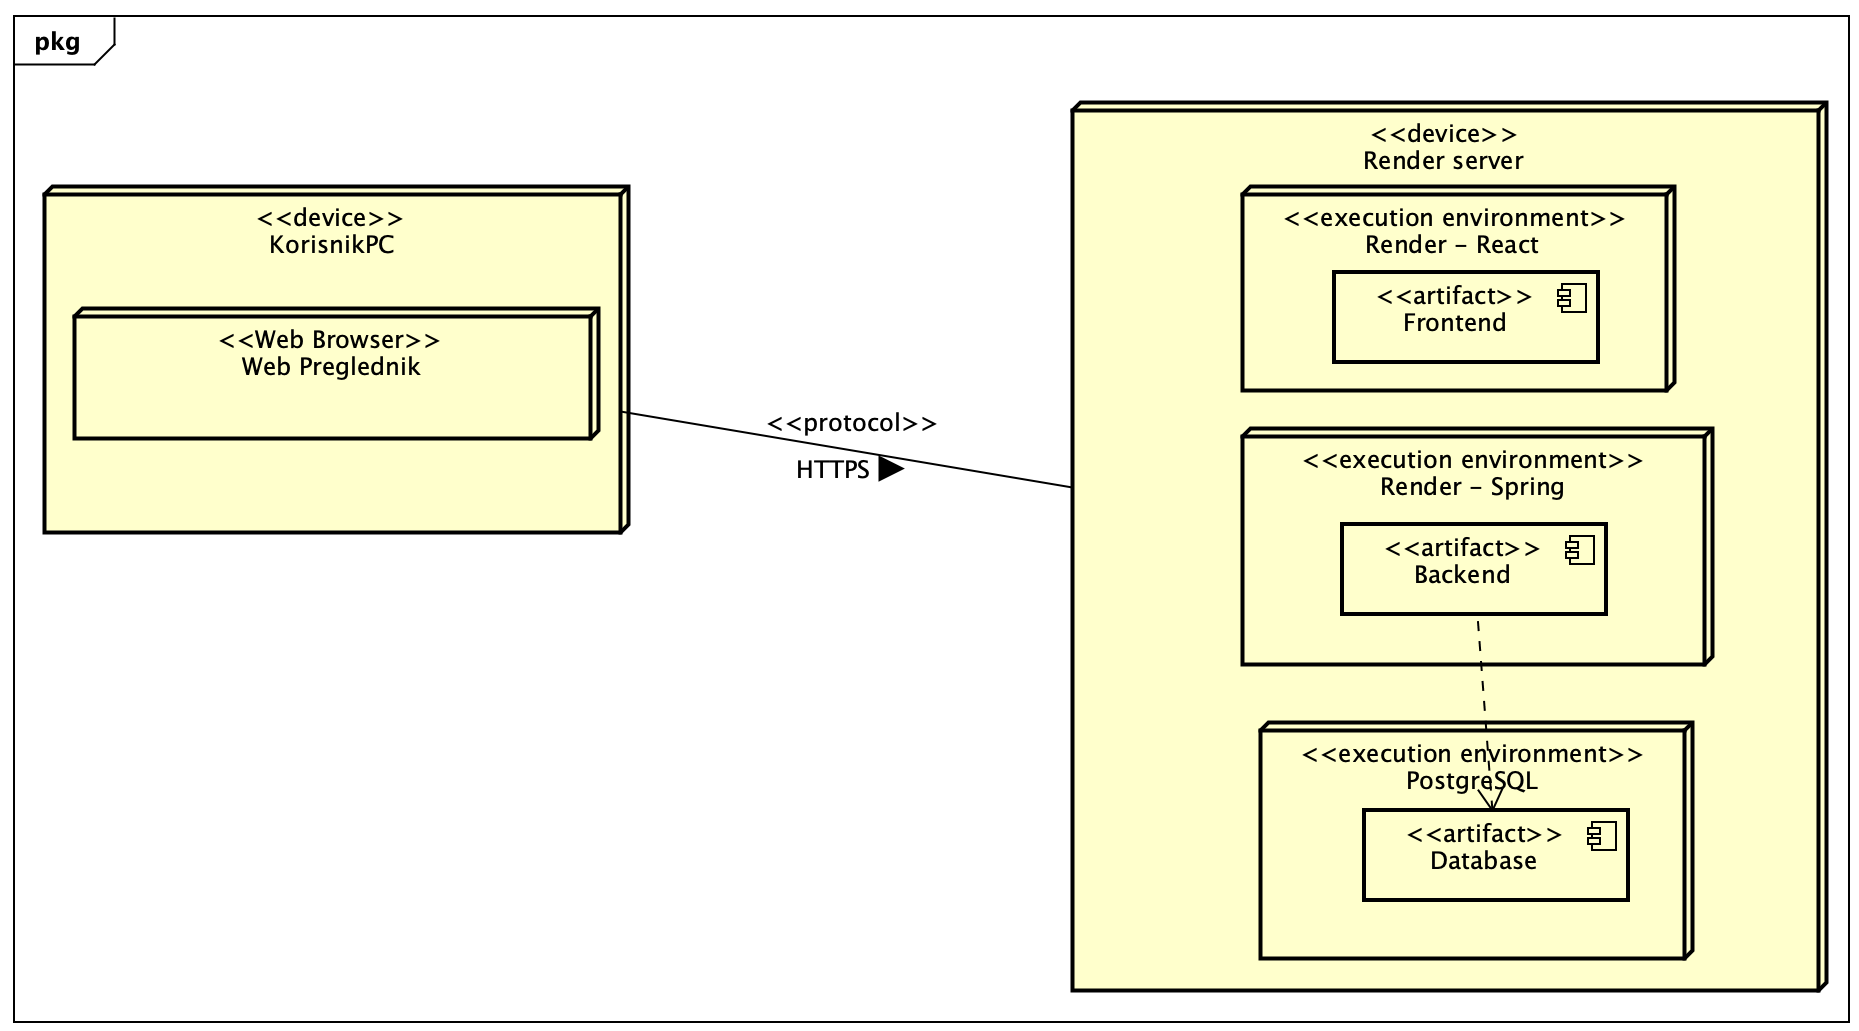
\includegraphics[scale=0.45]{dijagrami/dijagramRazmjestaja.png}
			 	\centering
			 	\caption{Dijagram razmještaja}
			 	\label{fig:promjene}
			 \end{figure}
			
			\eject 
		
		\section{Upute za puštanje u pogon}
		
			U ovom poglavlju opisat ćemo postupak puštanja web aplikacije u pogon - na koji način se od izvornog koda dolazi do potpuno postavljene baze podataka i poslužitelja koji odgovara na upite korisnika. U ovom postupku posebno ćemo opisat postavljanje baze podataka, backend poslužitelja i frontend poslužitelja. Za puštanje aplikacije u pogon preporuča se korištenje pružatelja servera te smo se odlučili za Render.
			
			\textbf{Kreiranje baze podataka}
			
			Za postavljanje baze podataka u Render-u potrebno je pratiti sljedeće korake:
			
			\begin{packed_enum}
				
				\item  U padajućem izborniku "New" izabrati opciju "PostgreSQL"
				\item	Postaviti ime baze podataka te korisničko ime (username) za korisnika baze, lozinka je automatski generirana
				\item	U padajućem izborniku "Region" izabrati opciju "Frankfurt"
				\item	Odabrati opciju "Create database", u slučaju odabira besplatnog plana valja napomenuti da ima maksimalnu pohranu podataka do 1GB te da se baza podataka briše nakon 90 dana 

			\end{packed_enum}
		
			\begin{figure}[H]
				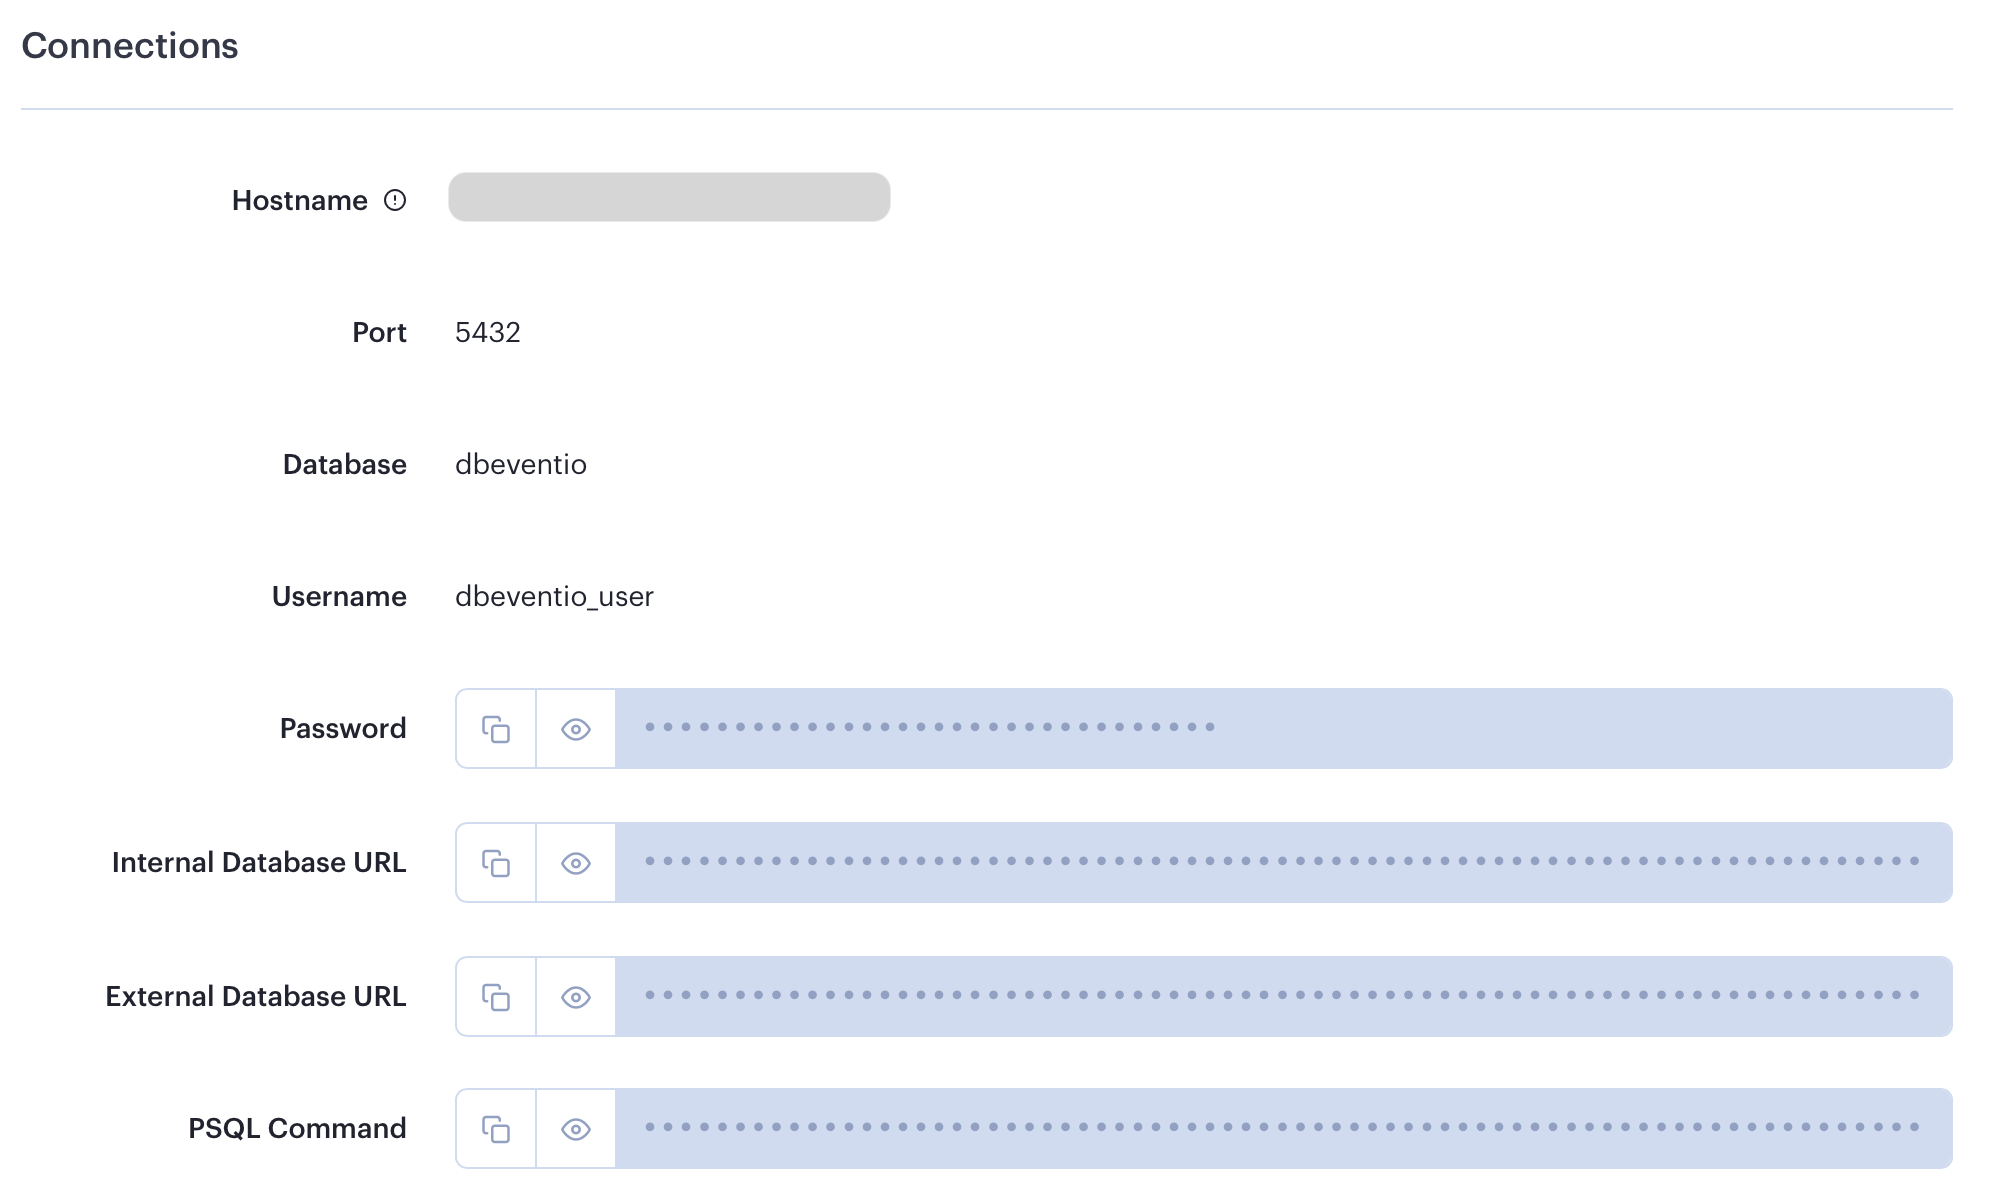
\includegraphics[scale=0.45]{deploy/baza.png}
				\centering
				\caption{Postavke PostgreSQL baze podataka nakon kreiranja}
				\label{fig:promjene}
			\end{figure}
			
			\textbf{Kreiranje backenda}
			
			Na slici 5.13. također su prikazane varijable koje će se koristiti za spajanje na backend poslužitelj što je opisano u sljedećim koracima.
			
			\begin{packed_enum}
				
				\item  U padajućem izborniku "New" izabrati opciju "Web Service"
				\item	Povezati GitHub račun te u odabrati odgovarajući projekt za povezivanje
				\item	Postaviti ime koje će također biti postati i dio web adrese
				\item	Opciju "Root directory" ostaviti praznom te postaviti "Environment - Docker"
				\item 	U padajućem izborniku "Region" izabrati opciju "Frankfurt"
				\item 	Na dnu stranice proširiti opciju "Advanced"
				\item 	Dodati potrebne environment varijable koje se trebaju kopirati iz postavki baze podataka na Render, slika 5.13.
				
				\begin{figure}[H]
					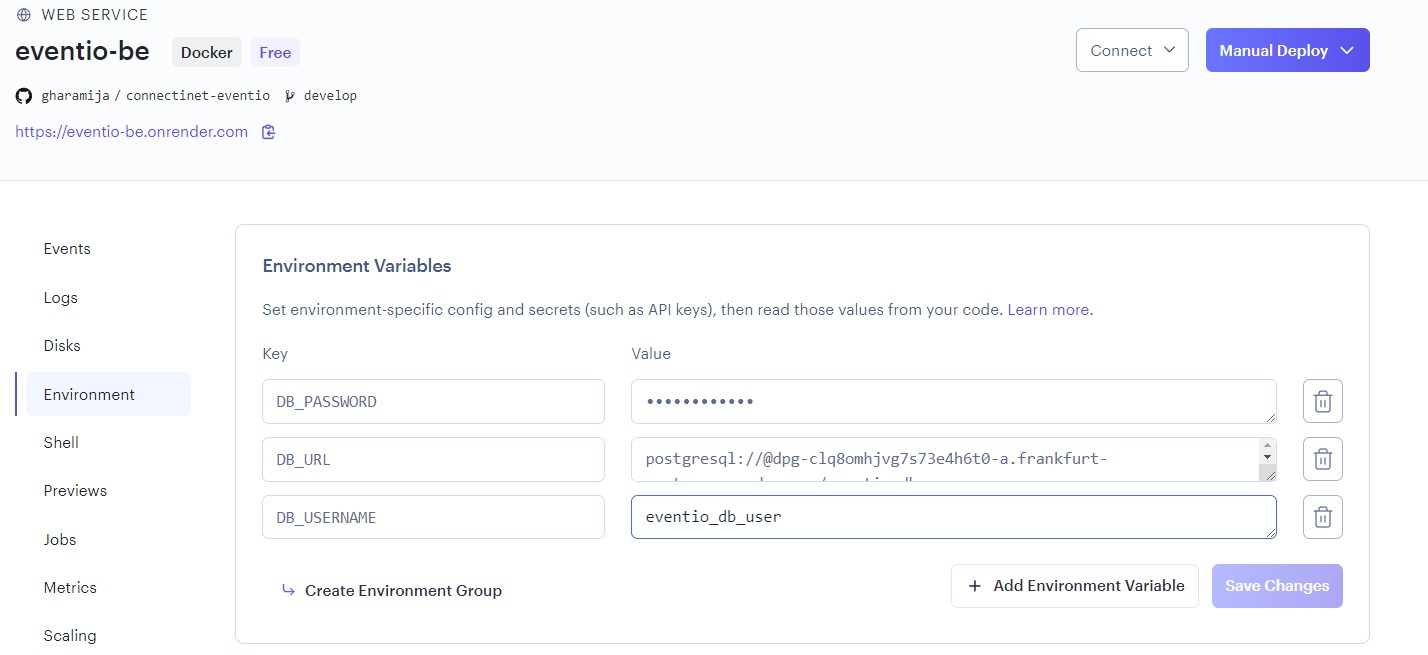
\includegraphics[scale=0.3]{deploy/backendEnv.jpeg}
					\centering
					\caption{Environment varijable za backend}
					\label{fig:promjene}
				\end{figure}
				
				\item 	Postaviti putanju na Dockerfile (ovisno o packet manageru), u našem slučaju to je "./docker/maven/Dockerfile"
				
				Ovdje prilažemo slike koje prikazuju kofiguracijske postavke na Renderu, Dockerfile na spomenutoj putanji te dio datoteke 
				
				\begin{figure}[H]
					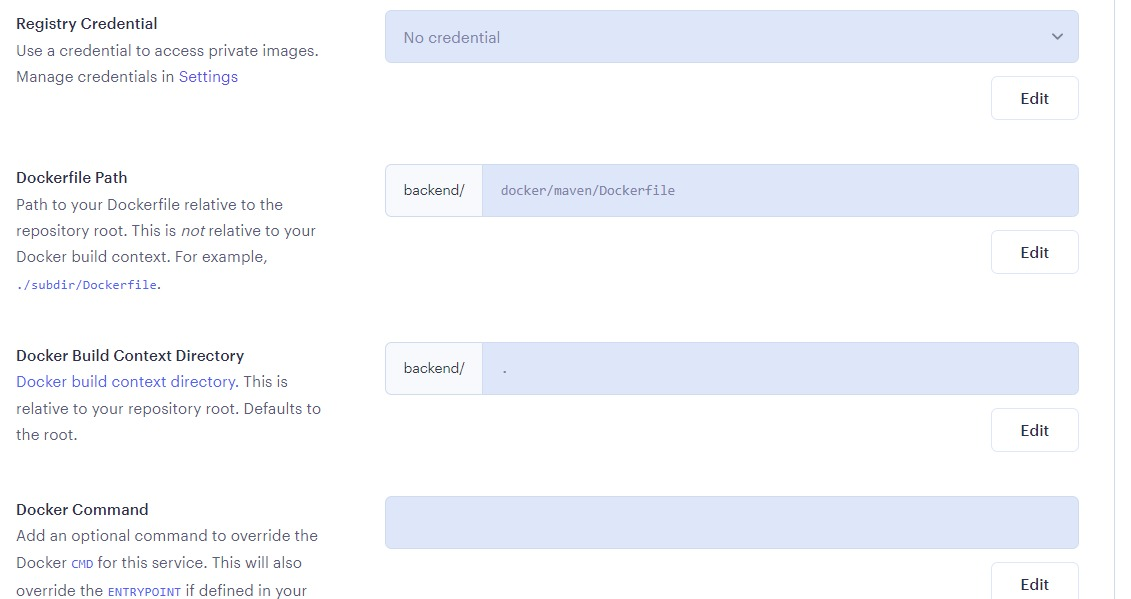
\includegraphics[scale=0.4]{deploy/backendConf.jpeg}
					\centering
					\caption{Konfiguracijske postavke backend poslužitelja}
					\label{fig:promjene}
				\end{figure}
				
				\begin{figure}[H]
					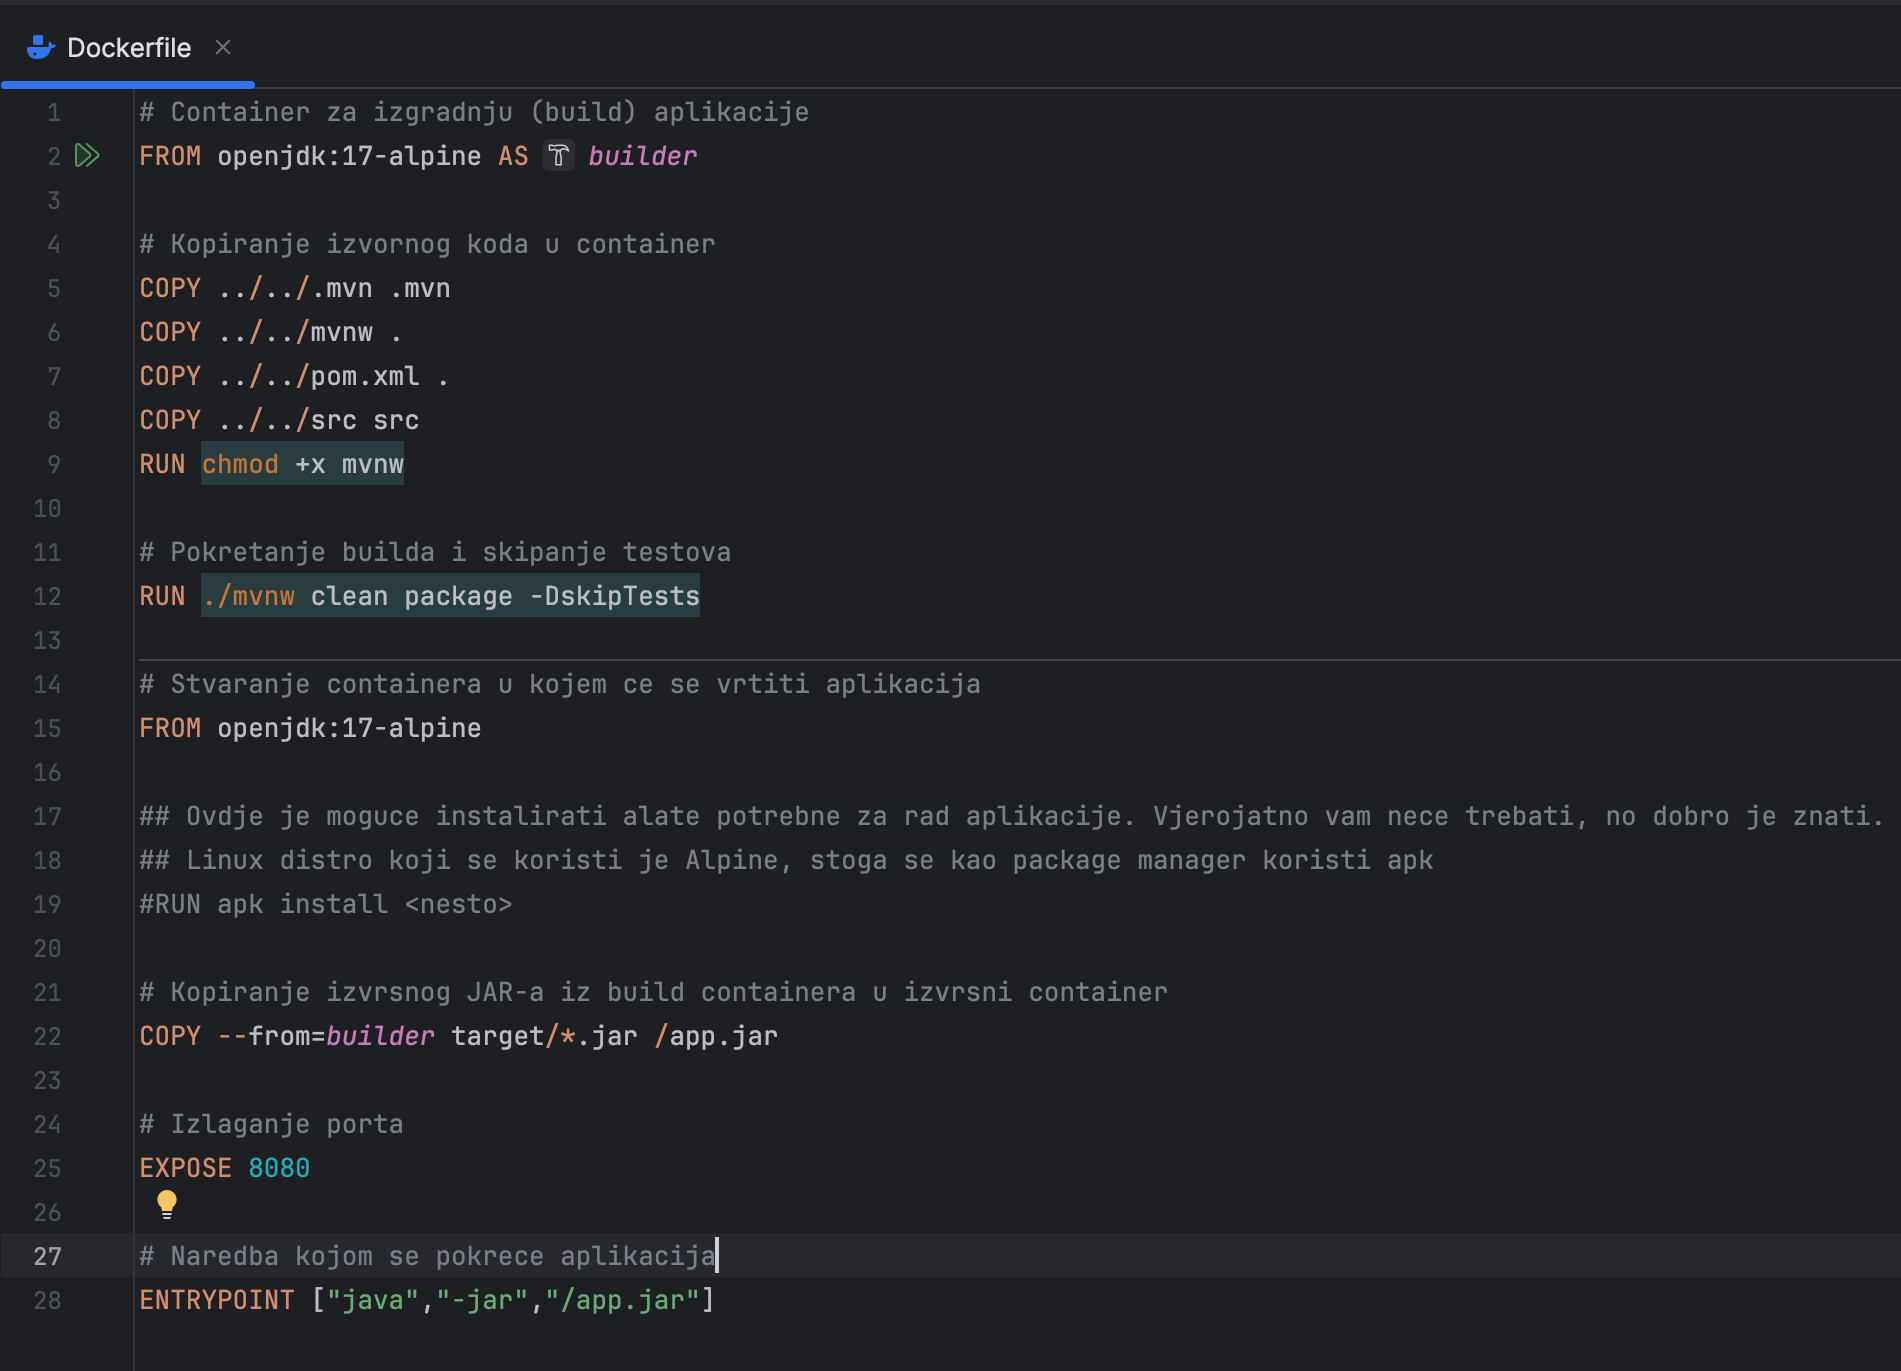
\includegraphics[scale=0.45]{deploy/dockerFile.png}
					\centering
					\caption{Dockerfile na putanju /docker/maven/Dockerfile}
					\label{fig:promjene}
				\end{figure}
				
				\item 	Odabrati opciju "Create Web Service"
				
				Ovdje napominjemo da u slučaju korištenja besplate verzije, nakon neaktivnosti aplikacije ona će biti automatski ugašena te ponovno podignuta zaprimanjem prvog zahtjeva. Drugim riječima, ovo može rezultirati sa nekoliko minuta nedostupnosti aplikacije nakon perioda neaktivnosti.
				
			\end{packed_enum}


			\textbf{Kreiranje frontenda}
			
			\begin{packed_enum}
				
				\item  U padajućem izborniku "New" izabrati opciju "Web Service"
				\item	Povezati GitHub račun te u odabrati odgovarajući projekt za povezivanje
				\item	Postaviti ime koje će također biti postati i dio web adrese
				\item	Opciju "Root directory" ostaviti praznom te postaviti "Environment - Node"
				\item 	U padajućem izborniku "Region" izabrati opciju "Frankfurt"
				\item 	Opciju "Build command" postaviti na "npm run build"
				\item 	Opciju "Start command" postaviti na "npm run start-prod"
				
				\begin{figure}[H]
					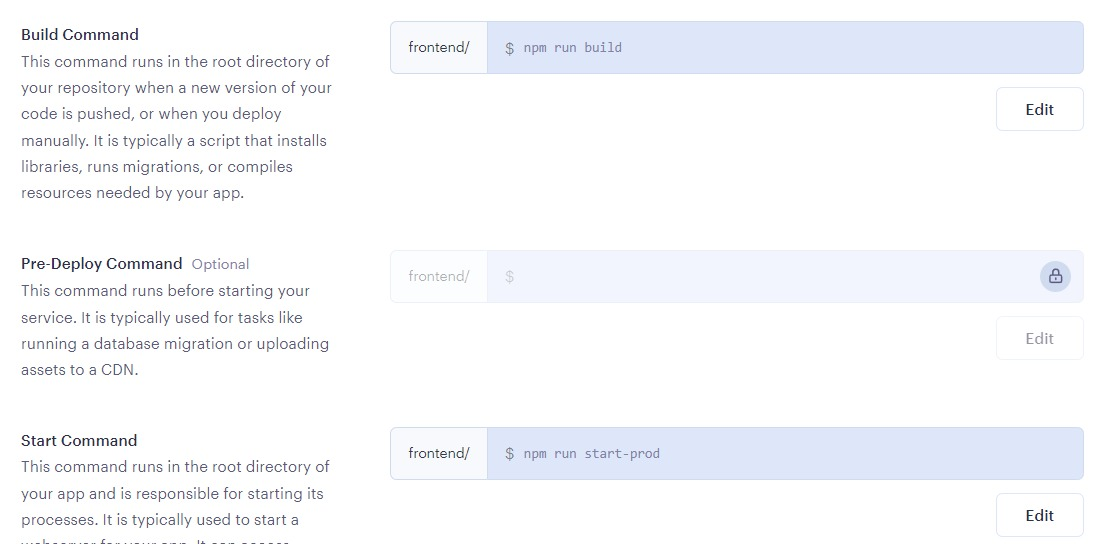
\includegraphics[scale=0.4]{deploy/frontendConf.jpeg}
					\centering
					\caption{Konfiguracijske postavke frontend poslužitelja}
					\label{fig:promjene}
				\end{figure}
				
				\item 	Na dnu stranice proširiti opciju "Advanced"
				\item 	Dodati potrebne environment varijable, "API-BASE-URL" postaviti na adresu podignutog backenda što je prikazano Render Dashboardu
				
				\begin{figure}[H]
					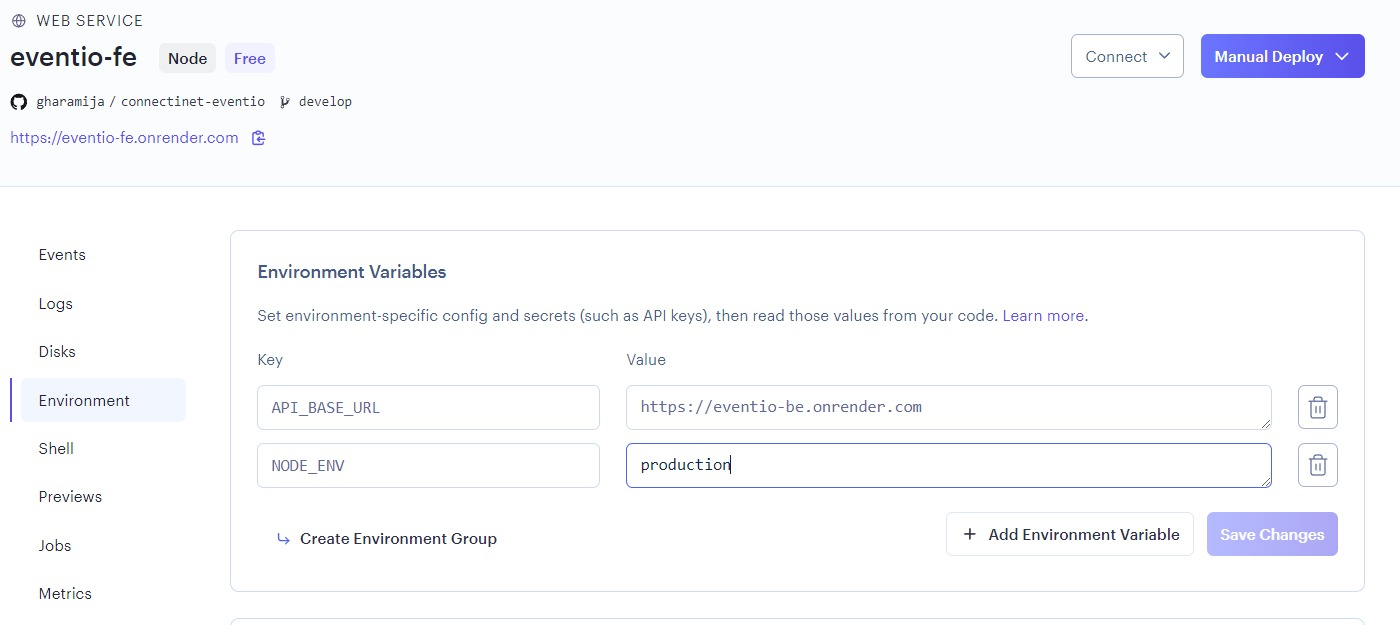
\includegraphics[scale=0.25]{deploy/frontendEnv.jpeg}
					\centering
					\caption{Environment varijable za frontend}
					\label{fig:promjene}
				\end{figure}
				
				\item 	Odabrati opciju "Create Web Service"
				
				
			\end{packed_enum}
			
			
			\eject 